\documentclass[11pt]{scrartcl}
\usepackage{dominatrix}
\usepackage{solarized-light}
\lstset{
language=R
}
\renewcommand\thesection{Problem \arabic{section}}
\renewcommand\thesubsection{\thesection (\alph{subsection})}
\renewcommand\thesubsubsection{(\roman{subsubsection})}

\title{Homework 6}
\subject{Intro to Financial Engineering IEOR W4700}
\author{Linan Qiu\\\texttt{lq2137}}
\begin{document}
\maketitle

\section{}

\subsection{}

To find $q$,

\begin{lstlisting}
q_prob = function(r, delta_t, sigma) {
  u = exp(sigma*sqrt(delta_t))
  d = exp(-sigma*sqrt(delta_t))
  
  return((exp(r*delta_t) - d)/(u-d))
}
\end{lstlisting}

To build the stock tree,

\begin{lstlisting}
build_stock_tree = function(S, sigma, delta_t, N) {
  tree = matrix(0, nrow=N+1, ncol=N+1)
  
  u = exp(sigma*sqrt(delta_t))
  d = exp(-sigma*sqrt(delta_t))
  
  for (i in 1:(N+1)) {
    for (j in 1:i) {
      tree[i,j] = S * u^(j-1) * d^((i-1)-(j-1))
    }
  }
  return(tree)
}
\end{lstlisting}

To value the binomial option using the stock tree generated,

\begin{lstlisting}
value_binomial_option = function(tree, sigma, delta_t, r, X, type) {
  q = q_prob(r, delta_t, sigma)

  option_tree = matrix(0, nrow=nrow(tree), ncol=ncol(tree))
  if(type == 'put') {
    option_tree[nrow(option_tree),] = pmax(X - tree[nrow(tree),], 0)
  } else {
    option_tree[nrow(option_tree),] = pmax(tree[nrow(tree),] - X, 0)
  }

  for (i in (nrow(tree)-1):1) {
    for(j in 1:i) {
      option_tree[i, j] = ((1-q)*option_tree[i+1,j] + q*option_tree[i+1,j+1])/exp(r*delta_t)
    }
  }
  return(option_tree)
}
\end{lstlisting}

Putting this all together,

\begin{lstlisting}
binomial_option = function(type, sigma, T, r, X, S, N) {
  q = q_prob(r=r, delta_t=T/N, sigma=sigma)
  tree = build_stock_tree(S=S, sigma=sigma, delta_t=T/N, N=N)
  option = value_binomial_option(tree, sigma=sigma, delta_t=T/N, r=r, X=X, type=type)
  delta = (option[2,2]-option[2,1])/(tree[2,2]-tree[2,1])
  return(list(q=q, stock=tree, option=option, price=option[1,1], delta=delta))
}
\end{lstlisting}

I coded this manually because none of the \texttt{R} packages (\texttt{fOption}, \texttt{m4fe}) seem to work (and be able to replicate the numbers on the slides). They also don't show the entire tree. So I coded my own. This code for Binomial European Option Pricing is (I made it open source) at \url{https://github.com/linanqiu/binomial-european-option-r}.

Using the variables in the question,

\begin{lstlisting}
> binomial_option(type='put', sigma=0.33, T=1/4, r=0.05, X=48, S=50, N=3)
$q
[1] 0.4980841

$stock
         [,1]     [,2]     [,3]     [,4]
[1,] 50.00000  0.00000  0.00000  0.00000
[2,] 45.45670 54.99739  0.00000  0.00000
[3,] 41.32623 50.00000 60.49427  0.00000
[4,] 37.57108 45.45670 54.99739 66.54054

$option
          [,1]      [,2] [,3] [,4]
[1,]  2.247762 0.0000000    0    0
[2,]  3.866524 0.6353901    0    0
[3,]  6.474186 1.2712151    0    0
[4,] 10.428919 2.5433006    0    0

$price
[1] 2.247762

$delta
[1] -0.3386687
\end{lstlisting}

The option price is $2.247762$

\subsection{}

Shortcut function to calculate $\Delta$ from the tree produced by \texttt{binomial\_option}:

\begin{lstlisting}
delta = function(binomial_option, row, col) {
  stock_tree = binomial_option$stock
  option_tree = binomial_option$option
  return((option_tree[row+1, col+1] - option_tree[row+1, col])/(stock_tree[row+1, col+1] - stock_tree[row+1, col]))
}
\end{lstlisting}

\begin{itemize}
\item At start, $S=50$, so $\Delta = \dfrac{C_U-C_D}{S_U-S_D} = \dfrac{0.6353901 - 3.866524}{54.99739-45.45670} = -0.3386687$. However, this $\Delta$ is for buying a put. If we are selling (writing) a put, we use $-\Delta$ stocks, hence $0.3386687$ stocks.
\item If stock went up, we are at $S=54.99739$ and $C = 0.6353901$. Then, $\Delta = \dfrac{0 - 1.2712151}{60.49427 - 50.00000} = -0.1211343$. Again, We use $-\Delta$ stocks, hence need $0.1211343$ stocks.
\item Now that stock went down, we are at $S=50$, $C=1.2712151$. Then $\Delta = \dfrac{0 - 2.5433006}{54.99739 - 45.45670} = -0.266574$. We use $-\Delta$ stocks, hence need $0.266574$ stocks.
\end{itemize}


\section{}

\subsection{}

\begin{lstlisting}
> binomial_option(type='call', sigma=0.33, T=1, r=0.1, X=100, S=100, N=6)
$q
[1] 0.5285562

$stock
          [,1]      [,2]      [,3]     [,4]     [,5]     [,6]     [,7]
[1,] 100.00000   0.00000   0.00000   0.0000   0.0000   0.0000   0.0000
[2,]  87.39589 114.42186   0.00000   0.0000   0.0000   0.0000   0.0000
[3,]  76.38041 100.00000 130.92361   0.0000   0.0000   0.0000   0.0000
[4,]  66.75334  87.39589 114.42186 149.8052   0.0000   0.0000   0.0000
[5,]  58.33968  76.38041 100.00000 130.9236 171.4099   0.0000   0.0000
[6,]  50.98648  66.75334  87.39589 114.4219 149.8052 196.1304   0.0000
[7,]  44.56009  58.33968  76.38041 100.0000 130.9236 171.4099 224.4161

$option
          [,1]      [,2]      [,3]     [,4]     [,5]     [,6]     [,7]
[1,] 17.275347  0.000000  0.000000  0.00000  0.00000  0.00000   0.0000
[2,]  7.944699 26.147082  0.000000  0.00000  0.00000  0.00000   0.0000
[3,]  2.257886 13.269646 38.464454  0.00000  0.00000  0.00000   0.0000
[4,]  0.000000  4.343593 21.653136 54.68229  0.00000  0.00000   0.0000
[5,]  0.000000  0.000000  8.355956 34.20200 74.68832  0.00000   0.0000
[6,]  0.000000  0.000000  0.000000 16.07471 51.45809 97.78328   0.0000
[7,]  0.000000  0.000000  0.000000  0.00000 30.92361 71.40993 124.4161

$price
[1] 17.27535

$delta
[1] 0.6735146
\end{lstlisting}

\subsection{}

\begin{lstlisting}
> binomial_option(type='put', sigma=0.33, T=1, r=0.1, X=100, S=100, N=6)
$q
[1] 0.5285562

$stock
          [,1]      [,2]      [,3]     [,4]     [,5]     [,6]     [,7]
[1,] 100.00000   0.00000   0.00000   0.0000   0.0000   0.0000   0.0000
[2,]  87.39589 114.42186   0.00000   0.0000   0.0000   0.0000   0.0000
[3,]  76.38041 100.00000 130.92361   0.0000   0.0000   0.0000   0.0000
[4,]  66.75334  87.39589 114.42186 149.8052   0.0000   0.0000   0.0000
[5,]  58.33968  76.38041 100.00000 130.9236 171.4099   0.0000   0.0000
[6,]  50.98648  66.75334  87.39589 114.4219 149.8052 196.1304   0.0000
[7,]  44.56009  58.33968  76.38041 100.0000 130.9236 171.4099 224.4161

$option
          [,1]      [,2]      [,3]         [,4] [,5] [,6] [,7]
[1,]  7.759088  0.000000  0.000000 0.000000e+00    0    0    0
[2,] 12.553251  3.729666  0.000000 0.000000e+00    0    0    0
[3,] 19.428170  6.820344  1.091538 0.000000e+00    0    0    0
[4,] 28.369599 12.070646  2.354221 1.416430e-15    0    0    0
[5,] 38.381932 20.341195  5.077566 3.054946e-15    0    0    0
[6,] 47.360665 31.593802 10.951256 6.588884e-15    0    0    0
[7,] 55.439912 41.660322 23.619585 1.421085e-14    0    0    0

$price
[1] 7.759088

$delta
[1] -0.3264854
\end{lstlisting}

\subsection{}

To satisfy put call parity, let $C_C$ be price of call option and $C_P$ be price of put option. Then, buying a call and selling a put should give us the same cash flow as a forward on the underlier.

\begin{align*}
C_C - C_P &= S - \frac{X}{e^r} \\
17.27535 - 7.759088 &= 100 - \frac{100}{e^{0.1}} \\
9.516258 &= 9.516258
\end{align*}


\section{}

Program written in above sections. Code is available at \url{https://github.com/linanqiu/binomial-european-option-r}.

\begin{lstlisting}
periods = seq(100, 120)
option_price_vary_period = function(period) {
  print(period)
  option = binomial_option(type='call', sigma=0.2, T=1, r=0, X=100, S=100, N=period)
  return(option$price)
}
values = sapply(periods, option_price_vary_period)
library(ggplot2)
data = as.data.frame(list(periods=periods, values=values))
plot = ggplot(data=data) + geom_line(aes(x=periods, y=values)) + labs(title="Call Value", x="Periods", y="Value")
plot
\end{lstlisting}

\begin{figure}[H]
\centering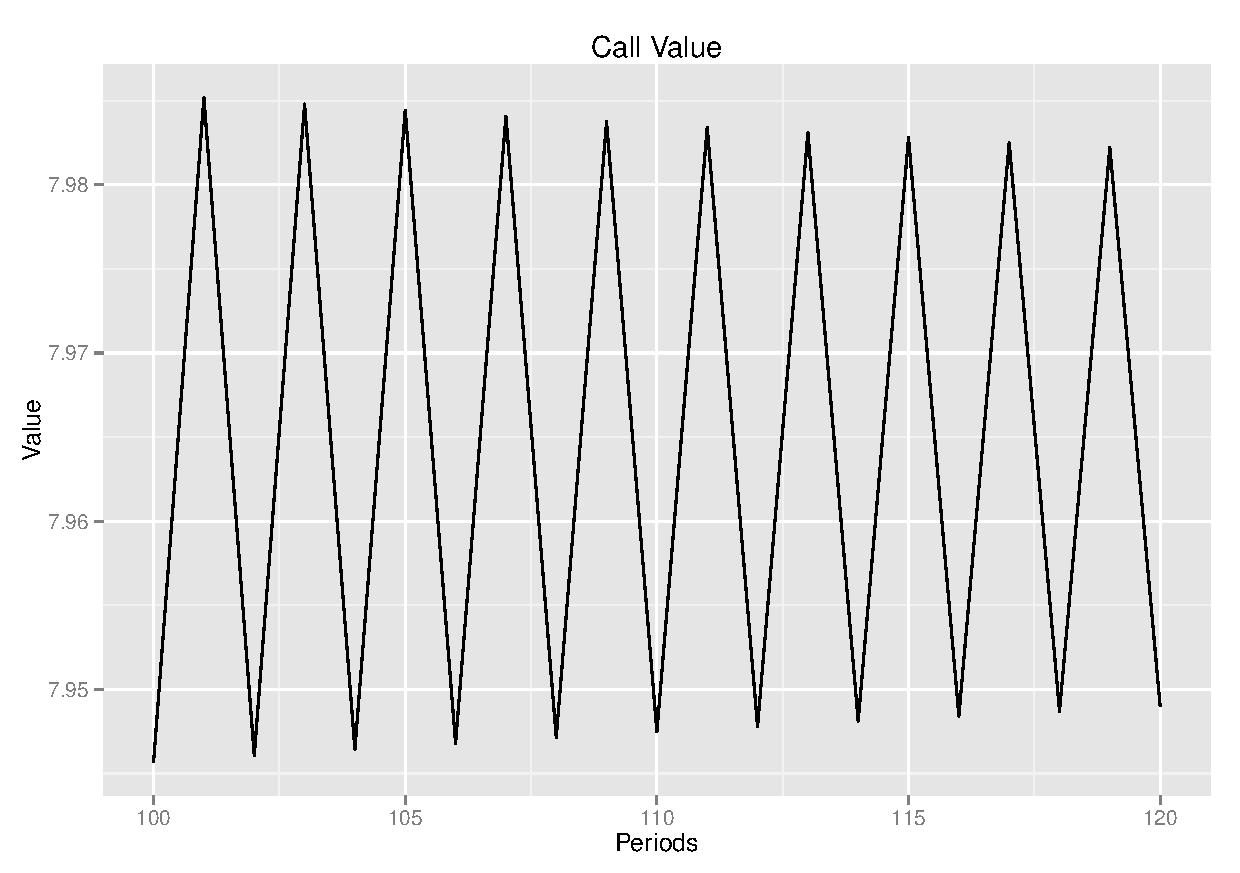
\includegraphics[width=\textwidth]{./hw6/problem3-120.pdf}
\caption{Plot of call option value calculated using the function above against periods (from 100 to 120)}
\end{figure}

Why do 100 to 120 when one can do more!

\begin{figure}[H]
\centering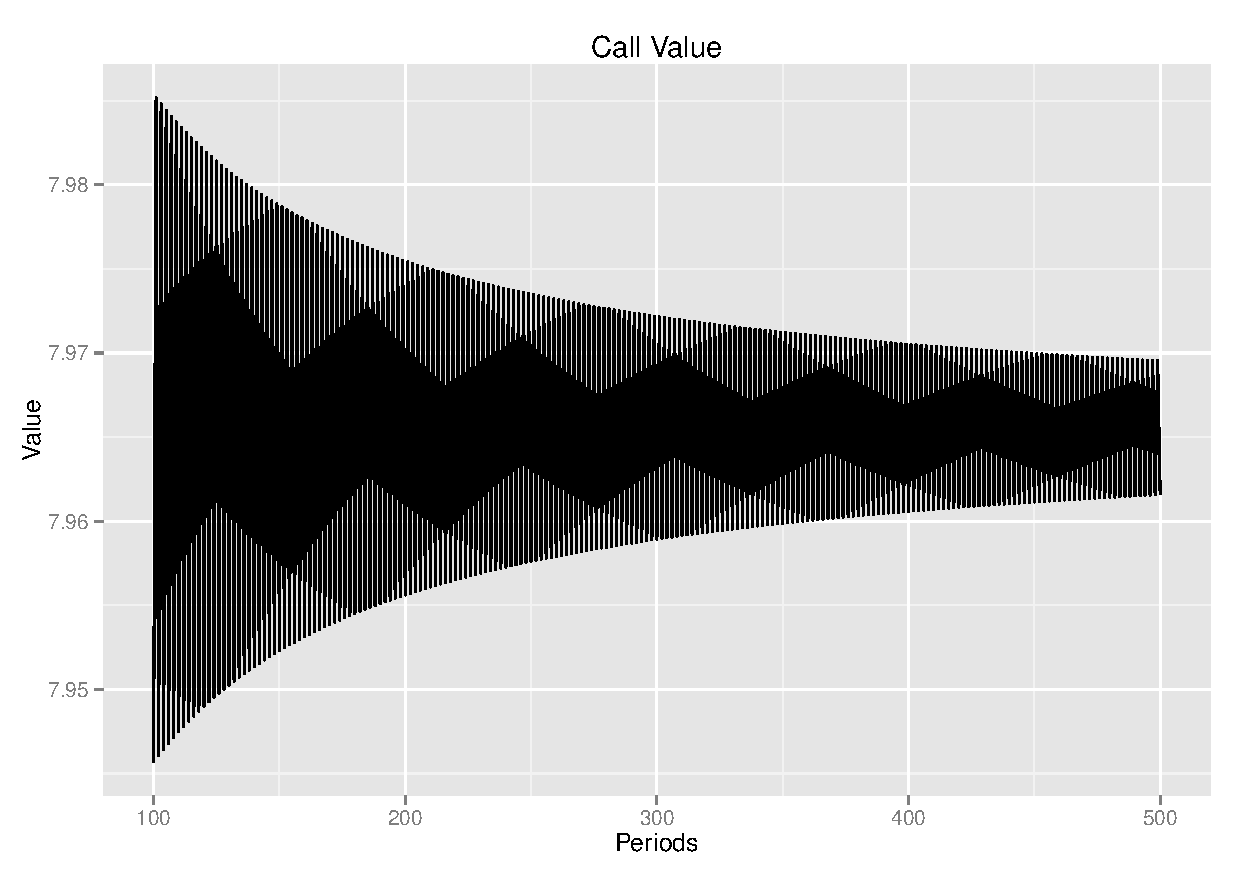
\includegraphics[width=\textwidth]{./hw6/problem3-500.pdf}
\caption{Plot of call option value calculated using the function above against periods (from 100 to 500). Also this is pretty pretty. After 500 the code becomes a little slow since I'm generating $N^2$ matrices.}
\end{figure}

Okay I managed to speed it up by parallelizing it. Let's try a 1000 periods now (this took a minute on 8 CPU cores). The code is

\begin{lstlisting}
library(parallel)
cl = makeCluster(8)
clusterEvalQ(cl, source('binomial.R'))
periods = seq(100, 1000)
periods = sample(periods)
valuesPar = parSapply(cl=cl, periods, option_price_vary_period)
data = as.data.frame(list(periods=periods, values=valuesPar))
plot = ggplot(data=data) + geom_line(aes(x=periods, y=values)) + labs(title="Call Value", x="Periods", y="Value")
plot
stopCluster(cl)
\end{lstlisting}

\begin{landscape}
\begin{figure}[H]
\centering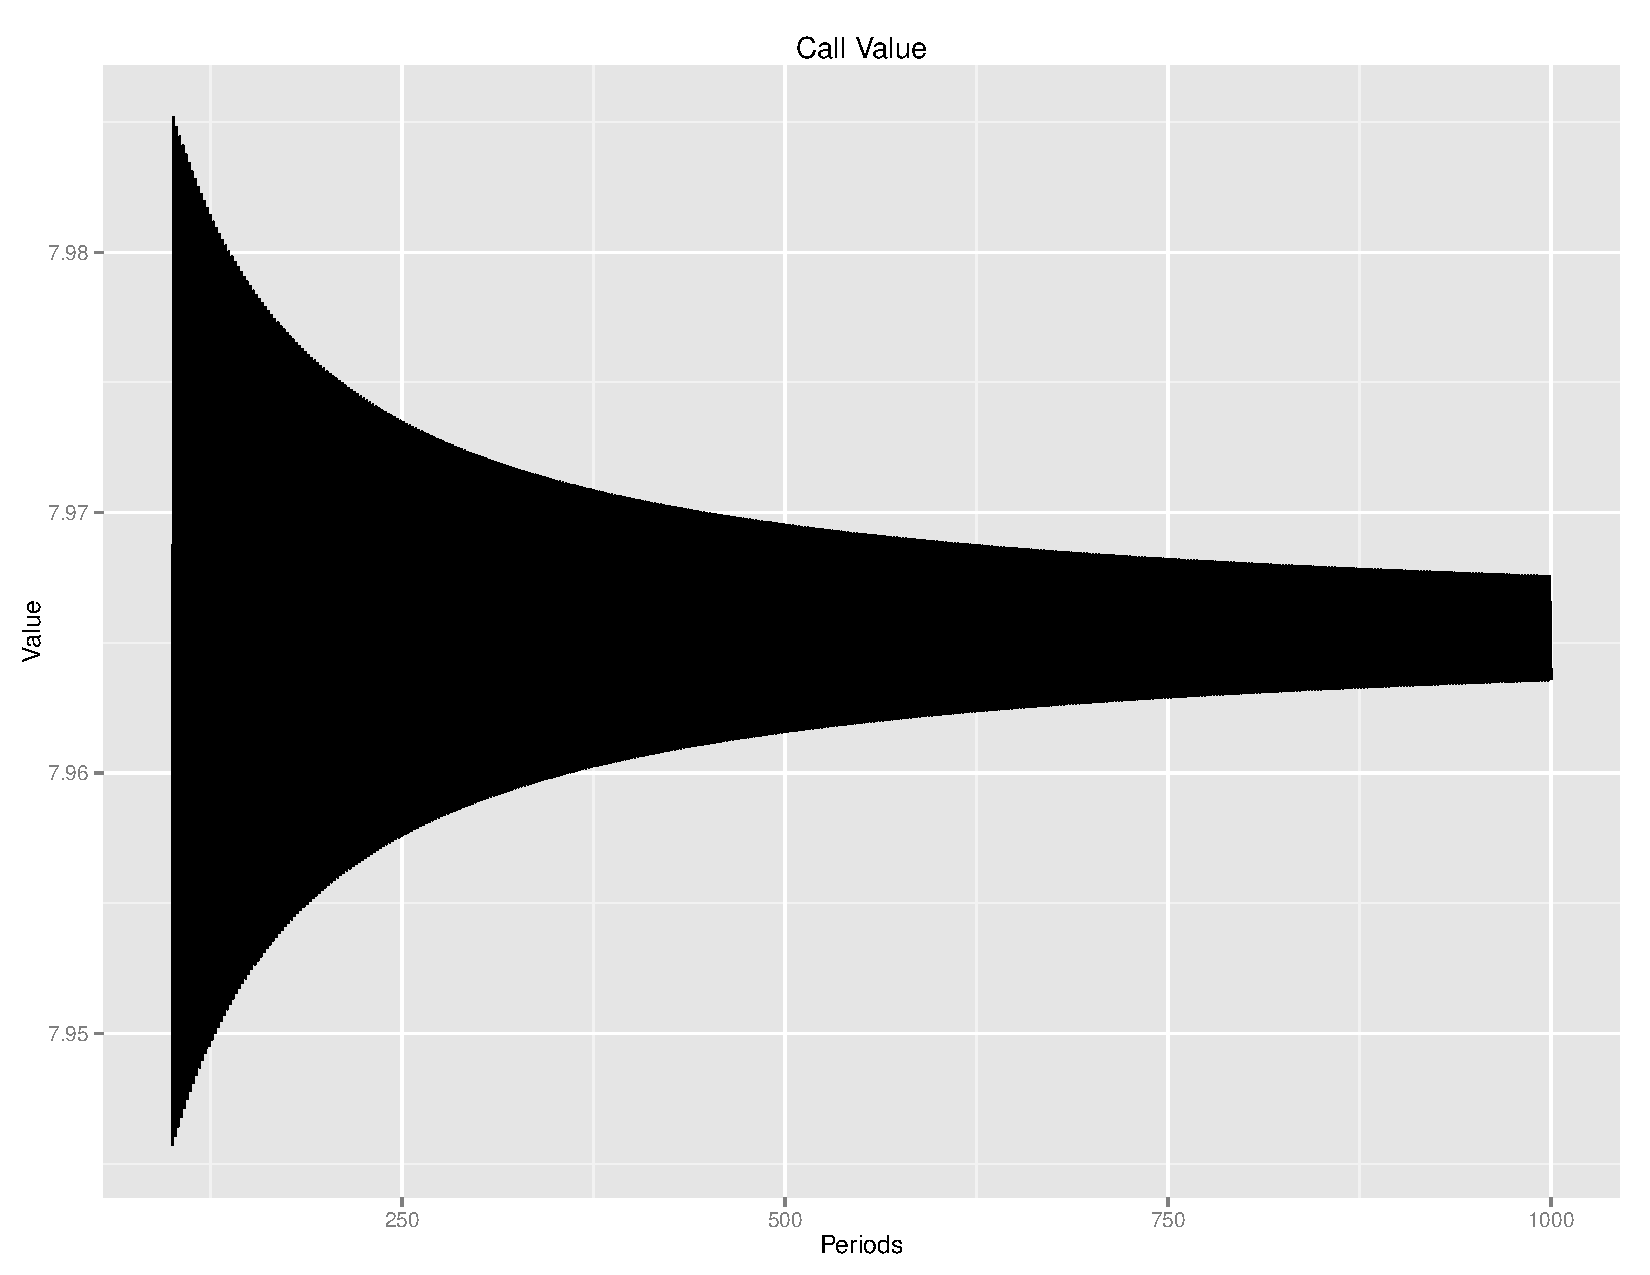
\includegraphics[width=1.15\textwidth]{./hw6/problem3-1000.pdf}
\caption{Plot of call option value calculated using the function above against periods (from 100 to 1000). This is almost beautiful.}
\end{figure}
\end{landscape}

\section{}

Build the tree manually. Let's find $q$ the risk neutral ``probability'' first.

\[S = 50 = \frac{qS_U + (1-q)S_D}{R} = \frac{q55 + (1-q)45}{e^{0.1*0.5}}\]

Solving for $q$, $q = 0.7563555$

\begin{lstlisting}
> uniroot(function(q) {(q*55 + (1-q)*45)/exp(0.1*0.5) - 50}, interval=c(-1, 1))
$root
[1] 0.7563555

$f.root
[1] 0

$iter
[1] 1

$init.it
[1] NA

$estim.prec
[1] 1.756355
\end{lstlisting}

Then,

\[P = \frac{qP_U + (1-q)P_D}{R} = \frac{0 + (1-0.7563555)(50-45)}{e^{0.1*0.5}} = 1.158809\]

To verify this (since I'm revising for the midterm anyway), let's replicate the riskless bond. Consider a portfolio with $\Delta$ stocks and $1$ put.

\begin{itemize}
\item When $S_U = 55$, $P_U = 0$. Portfolio is worth $\Delta 55$.
\item When $S_D = 45$, $P_D = 5$. Portfolio is worth $\Delta 45 + 5$.
\end{itemize}

\[\Delta 55 = \Delta 45 + 5\]

Then, $\Delta = 0.5$, ie. we must long $0.5$ stocks. The value of both portfolios are

\begin{itemize}
\item When $S_U = 55$, $P_U = 0$. Portfolio is worth $\Delta 55 = 27.5$.
\item When $S_D = 45$, $P_D = 5$. Portfolio is worth $\Delta 45 + 5 = 27.5$.
\end{itemize}

That means the portfolio must be worth $\dfrac{27.5}{e^{0.1*0.5}} = 26.15881$ presently. That means

\[P + \Delta S = 26.15881 = P + 0.5(50)\]
\[P = 1.158809\]

The value of the put option is $1.158809$ which verifies the answer from using binomial trees.

\section{}

Let $D$ be the value of the derivative.

\[S = 50 = \frac{qS_U + (1-q)S_D}{R} = \frac{q27 + (1-q)23}{e^{0.1/6}}\]

Solving for $q$, $q = 0.6050396$

\begin{lstlisting}
> uniroot(function(q) {(q*27 + (1-q)*23)/exp(0.1/6) - 25}, interval=c(-1, 1))
$root
[1] 0.6050396

$f.root
[1] 0

$iter
[1] 1

$init.it
[1] NA

$estim.prec
[1] 1.60504
\end{lstlisting}

Then,

\[D = \frac{qD_U + (1-q)D_D}{R} = \frac{(0.6050396)27^2 + (1-0.6050396)23^2}{e^{0.1/6}} = 639.2642\]

Can be verified via portfolio replication method.

Suppose portfolio comprises $\Delta$ stocks and $1$ $D$.

\begin{itemize}
\item When $S_U = 27$, $D_U = 27^2$. Portfolio is worth $\Delta 27 + D_U$
\item When $S_D = 23$, $D_D = 23^2$. Portfolio is worth $\Delta 23 + D_D$
\end{itemize}

\begin{align*}
\Delta 27 + D_U &= \Delta 23 + D_D \\
\Delta 27 + 27^2 &= \Delta 23 + 23^2 \\
\Delta &= -50
\end{align*}

We short $50$ stocks. Then in both states, portfolio is worth $\Delta 27 + 27^2 = -621 = \Delta 23 + 23^2$ Then the value of both portfolios before two months is $\dfrac{\Delta 27 + 27^2}{e^{0.1/6}} = -610.7358$.

\[D + \Delta S = D -50(25) = -610.7358\]
\[D = 639.2642\]

Verifies the answer above.

\end{document}
